\PassOptionsToPackage{unicode=true}{hyperref} % options for packages loaded elsewhere
\PassOptionsToPackage{hyphens}{url}
\PassOptionsToPackage{dvipsnames,svgnames*,x11names*}{xcolor}
%
\documentclass[
  a4paper,
  twoside]{article}
\usepackage{lmodern}
\usepackage{amssymb,amsmath}
\usepackage{ifxetex,ifluatex}
\ifnum 0\ifxetex 1\fi\ifluatex 1\fi=0 % if pdftex
  \usepackage[T1]{fontenc}
  \usepackage[utf8]{inputenc}
  \usepackage{textcomp} % provides euro and other symbols
\else % if luatex or xelatex
  \usepackage{unicode-math}
  \defaultfontfeatures{Scale=MatchLowercase}
  \defaultfontfeatures[\rmfamily]{Ligatures=TeX,Scale=1}
  \setmainfont[]{Verdana}
\fi
% use upquote if available, for straight quotes in verbatim environments
\IfFileExists{upquote.sty}{\usepackage{upquote}}{}
\IfFileExists{microtype.sty}{% use microtype if available
  \usepackage[]{microtype}
  \UseMicrotypeSet[protrusion]{basicmath} % disable protrusion for tt fonts
}{}
\makeatletter
\@ifundefined{KOMAClassName}{% if non-KOMA class
  \IfFileExists{parskip.sty}{%
    \usepackage{parskip}
  }{% else
    \setlength{\parindent}{0pt}
    \setlength{\parskip}{6pt plus 2pt minus 1pt}}
}{% if KOMA class
  \KOMAoptions{parskip=half}}
\makeatother
\usepackage{xcolor}
\IfFileExists{xurl.sty}{\usepackage{xurl}}{} % add URL line breaks if available
\IfFileExists{bookmark.sty}{\usepackage{bookmark}}{\usepackage{hyperref}}
\hypersetup{
  pdftitle={Latex, YAML, RMarkdown},
  pdfauthor={Dortmunder Statistik},
  colorlinks=true,
  linkcolor=blue,
  filecolor=Maroon,
  citecolor=Blue,
  urlcolor=gray,
  breaklinks=true}
\urlstyle{same}  % don't use monospace font for urls
\usepackage[margin=1in]{geometry}
\usepackage{longtable,booktabs}
% Allow footnotes in longtable head/foot
\IfFileExists{footnotehyper.sty}{\usepackage{footnotehyper}}{\usepackage{footnote}}
\makesavenoteenv{longtable}
\usepackage{graphicx,grffile}
\makeatletter
\def\maxwidth{\ifdim\Gin@nat@width>\linewidth\linewidth\else\Gin@nat@width\fi}
\def\maxheight{\ifdim\Gin@nat@height>\textheight\textheight\else\Gin@nat@height\fi}
\makeatother
% Scale images if necessary, so that they will not overflow the page
% margins by default, and it is still possible to overwrite the defaults
% using explicit options in \includegraphics[width, height, ...]{}
\setkeys{Gin}{width=\maxwidth,height=\maxheight,keepaspectratio}
\setlength{\emergencystretch}{3em}  % prevent overfull lines
\providecommand{\tightlist}{%
  \setlength{\itemsep}{0pt}\setlength{\parskip}{0pt}}
\setcounter{secnumdepth}{5}
% Redefines (sub)paragraphs to behave more like sections
\ifx\paragraph\undefined\else
  \let\oldparagraph\paragraph
  \renewcommand{\paragraph}[1]{\oldparagraph{#1}\mbox{}}
\fi
\ifx\subparagraph\undefined\else
  \let\oldsubparagraph\subparagraph
  \renewcommand{\subparagraph}[1]{\oldsubparagraph{#1}\mbox{}}
\fi

% set default figure placement to htbp
\makeatletter
\def\fps@figure{htbp}
\makeatother

\setlength{\columnsep}{18pt}
\usepackage{multicol}
\newcommand{\hideFromPandoc}[1]{#1}
\hideFromPandoc{ \let\Begin\begin \let\End\end }
\definecolor{DoStat}{RGB}{4, 72, 145}
\usepackage{fancyhdr}
\pagestyle{fancy}
\fancyhf{}
\fancyhead[LE]{\itshape\nouppercase{\color{DoStat}\leftmark}}
\fancyhead[RO]{\itshape\nouppercase{\color{DoStat}\leftmark}}
\fancyfoot[LE]{\color{DoStat} \thepage \hspace{0.5cm} dortmunder\textbf{statistik}  • nr. 211 • jahresbericht 2018 • bevölkerung}
\fancyfoot[RO]{\color{DoStat} dortmunder\textbf{statistik}  • nr. 211 • jahresbericht 2018 • bevölkerung \hspace{0.5cm} \thepage}
\usepackage{graphicx}
\usepackage{booktabs}
\usepackage{longtable}
\usepackage{array}
\usepackage{multirow}
\usepackage{wrapfig}
\usepackage{float}
\usepackage{colortbl}
\usepackage{pdflscape}
\usepackage{tabu}
\usepackage{threeparttable}
\usepackage{threeparttablex}
\usepackage[normalem]{ulem}
\usepackage{makecell}
\usepackage{xcolor}

\title{Latex, YAML, RMarkdown}
\usepackage{etoolbox}
\makeatletter
\providecommand{\subtitle}[1]{% add subtitle to \maketitle
  \apptocmd{\@title}{\par {\large #1 \par}}{}{}
}
\makeatother
\subtitle{Options, packages and examples for PDF print}
\author{Dortmunder Statistik}
\date{}

\begin{document}
\maketitle

{
\hypersetup{linkcolor=}
\setcounter{tocdepth}{4}
\tableofcontents
}
\newpage

\begin {multicols}{2}

\hypertarget{wiki}{%
\section{Wiki}\label{wiki}}

\hypertarget{allgemeines}{%
\subsection{Allgemeines}\label{allgemeines}}

\hypertarget{yaml-settings-uxfcbersicht}{%
\subsubsection{YAML settings Übersicht}\label{yaml-settings-uxfcbersicht}}

\begin{itemize}
\tightlist
\item
  rmarkdown::default\_output\_format() zeigt die aktuelle YAML output Konfiguration
\end{itemize}

\begin{verbatim}
## $name
## [1] "bookdown::pdf_document2"
## 
## $options
## $options$...
## 
## 
## $options$keep_tex
## [1] TRUE
## 
## $options$latex_engine
## [1] "xelatex"
## 
## $options$toc
## [1] TRUE
## 
## $options$toc_depth
## [1] 4
\end{verbatim}

\hypertarget{template-info}{%
\subsubsection{Template Info}\label{template-info}}

\href{https://rstudio.github.io/rstudio-extensions/rmarkdown_templates.html}{R Markdown Document Templates}

\href{https://tex.stackexchange.com/questions/36/differences-between-luatex-context-and-xetex}{Latex engines}

\hypertarget{packages}{%
\subsection{packages}\label{packages}}

\hypertarget{r}{%
\subsubsection{R}\label{r}}

\hypertarget{rticles---vorlagen}{%
\paragraph{rticles - Vorlagen}\label{rticles---vorlagen}}

Templates und Vorlagen wissenschaftlicher Journals

\href{https://github.com/rstudio/rticles}{rtcles}

\hypertarget{ymlthis--yaml-package}{%
\paragraph{ymlthis- YAML package}\label{ymlthis--yaml-package}}

package zur vereinfachten Verwendung von YAML in RMarkdown und bookdown

\href{https://cran.r-project.org/web/packages/ymlthis/vignettes/introduction-to-ymlthis.html}{Einführung}

\href{https://cran.r-project.org/web/packages/ymlthis/ymlthis.pdf}{Reference Manual}

\href{https://cran.r-project.org/web/packages/ymlthis/vignettes/yaml-fieldguide.html}{YAML Field Guide}

\href{https://github.com/r-lib/ymlthis/blob/master/R/yml_latex.R}{yml\_latex.R}

\href{https://rdrr.io/github/r-lib/ymlthis/man/yml_latex_opts.html}{yml\_latex\_opts - Set LaTeX YAML options for PDF output}

\href{https://www.rdocumentation.org/packages/ymlthis/versions/0.1.2/topics/yml_resource_files}{yml\_resource\_files - Add external resource files to R Markdown document}

\href{https://github.com/r-lib/ymlthis/blob/master/R/yml_output.R}{yml\_output - Capture, validate, and write output YAML}

\hypertarget{bookdown}{%
\paragraph{bookdown}\label{bookdown}}

Authoring Books and Technical Documents with R Markdown

Single Page Documents \url{https://bookdown.org/yihui/bookdown/a-single-document.html}

customization \url{https://bookdown.org/yihui/bookdown/customization.html}

\hypertarget{latex}{%
\subsubsection{Latex}\label{latex}}

\hypertarget{multicol---mehrspaltige-layouts}{%
\paragraph{Multicol - mehrspaltige Layouts}\label{multicol---mehrspaltige-layouts}}

\url{https://www.ctan.org/pkg/multicol}

\url{https://tex.stackexchange.com/questions/8683/how-do-i-force-a-column-break-in-a-multi-column-page}

\url{https://stackoverflow.com/questions/40982836/latex-multicolumn-block-in-pandoc-markdown}

Mögliche Lösungen für 2 Spalten:
\url{https://github.com/yihui/rmarkdown-cookbook/issues/19}

Alternativen:

\url{https://stackoverflow.com/questions/34808612/how-make-2-column-layout-in-r-markdown-when-rendering-pdf}

\hypertarget{geometry---dokumentformatierung}{%
\paragraph{geometry - Dokumentformatierung}\label{geometry---dokumentformatierung}}

\href{https://ctan.org/pkg/geometry?lang=en}{Flexible and complete interface to document dimensions}

\href{http://mirrors.ctan.org/macros/latex/contrib/geometry/geometry-de.pdf}{Dokumentation}

ymlthis::yml\_latex\_opts() erlaubt die Einstellung über das package ymlthis zu konfigurieren

\hypertarget{pdfpages---einbindung-externe-pdf}{%
\paragraph{pdfpages - Einbindung externe PDF}\label{pdfpages---einbindung-externe-pdf}}

\href{https://ctan.org/pkg/pdfpages}{Einbindung von PDF Dokumenten in Latex}

\begin{itemize}
\tightlist
\item
  ggf. eine Lösung für Umschlag?
\end{itemize}

\hypertarget{koma-script---sammlung}{%
\paragraph{KOMA Script - Sammlung}\label{koma-script---sammlung}}

\href{https://www.ctan.org/pkg/koma-script}{package und class Sammlung}

\href{https://ctan.org/pkg/scrlayer-scrpage?lang=de}{inkl. Fußnoten package (z.Z. wird aber fancyhdr bevorzugt)}

\hypertarget{fancyhdr---kopf--fuuxdfzeile}{%
\paragraph{fancyhdr - Kopf- /Fußzeile}\label{fancyhdr---kopf--fuuxdfzeile}}

\href{https://ctan.org/pkg/fancyhdr?lang=de}{Kopf- und Fußzeilen}

\href{http://tug.ctan.org/tex-archive/macros/latex/contrib/fancyhdr/fancyhdr.pdf}{User Guide}

\href{https://bookdown.org/yihui/rmarkdown-cookbook/latex-header.html}{Abschnitt aus "bookdown}

\hypertarget{fontspec---schrift}{%
\paragraph{fontspec - Schrift}\label{fontspec---schrift}}

\href{https://www.ctan.org/pkg/fontspec}{Erweiterte Schrift Auswahl und Konfiguration}

\hypertarget{inhaltsverzeichnisse}{%
\paragraph{Inhaltsverzeichnisse}\label{inhaltsverzeichnisse}}

\hypertarget{tocloft---toc}{%
\subparagraph{tocloft - TOC}\label{tocloft---toc}}

\href{https://www.ctan.org/pkg/tocloft}{Erweiterte Optionen für Inhaltsverzeichnisse}

Beispiel \url{https://www.kronto.org/thesis/tips/format-toc.html}

\hypertarget{enumitem---toc}{%
\subparagraph{enumitem - TOC}\label{enumitem---toc}}

\href{https://ctan.org/pkg/enumitem?lang=de}{Manuelle Definition von TOCs}

\hypertarget{titlesec---uxfcberschriften}{%
\paragraph{titlesec - Überschriften}\label{titlesec---uxfcberschriften}}

\href{https://ctan.org/pkg/titlesec?lang=de}{Erweiterte Optionen für Überschriften}

\hypertarget{beispiele}{%
\subparagraph{Beispiele}\label{beispiele}}

\begin{itemize}
\tightlist
\item
  \url{https://tex.stackexchange.com/questions/225943/how-to-create-a-custom-table-of-contents}
\item
  \url{https://tex.stackexchange.com/questions/404103/customize-the-table-of-contents}
\item
  \url{https://cmry.github.io/notes/latextoc} - Sektionen ohne Nummerierung
\item
  \url{https://www.kronto.org/thesis/tips/format-toc.html}
\end{itemize}

\end {multicols}

\newpage

\hypertarget{formatierung}{%
\subsection{Formatierung}\label{formatierung}}

\hypertarget{pandoc-variablen}{%
\subsubsection{Pandoc Variablen}\label{pandoc-variablen}}

\href{https://pandoc.org/MANUAL.html\#variables-for-latex}{Anleitung}

\hypertarget{schriften}{%
\subsubsection{Schriften}\label{schriften}}

\href{https://tug.org/FontCatalogue/}{Schrift Katalog}

\hypertarget{seitenwechsel}{%
\subsubsection{Seitenwechsel}\label{seitenwechsel}}

Latex Page Breaks \url{https://web.archive.org/web/20100622022829/http://help-csli.stanford.edu/tex/latex-pagebreaks.shtml}

\hypertarget{logo-fuxfcr-titelseiten}{%
\subsubsection{Logo für Titelseiten}\label{logo-fuxfcr-titelseiten}}

\url{https://bookdown.org/yihui/rmarkdown-cookbook/latex-logo.html\#latex-logo}

Über includegraphics, Alternative siehe Latex package pdfpages

\hypertarget{nicht-nummerierte-kapitel}{%
\subsubsection{Nicht nummerierte Kapitel}\label{nicht-nummerierte-kapitel}}

\url{https://bookdown.org/yihui/rmarkdown-cookbook/unnumbered-sections.html}

\hypertarget{inhaltsverzeichnis}{%
\subsubsection{Inhaltsverzeichnis}\label{inhaltsverzeichnis}}

\href{https://texblog.org/2011/09/09/10-ways-to-customize-tocloflot/}{10 Wege Inhaltsverzeichnisse zu formatieren}

\hypertarget{farbpaletten}{%
\subsubsection{Farbpaletten}\label{farbpaletten}}

Neben frei zu definierenden Farben (siehe YAML xcolor settings, bzw. für \href{https://www.latextemplates.com/svgnames-colors}{Farbennamen} können Farben aus der Farbpalette ausgewählt werden

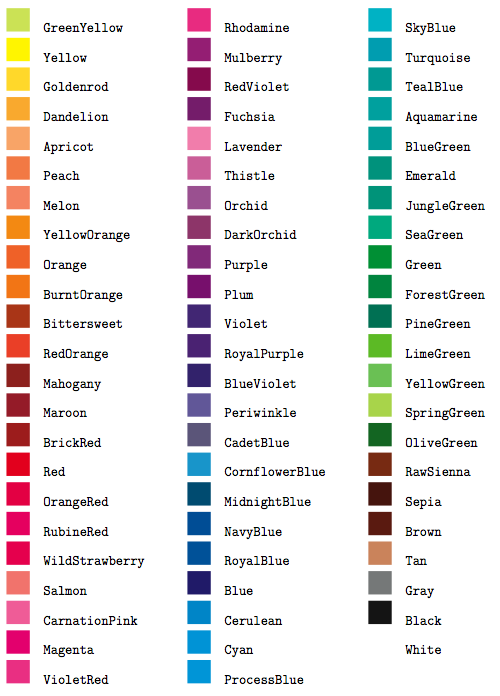
\includegraphics[width=30px]{latexcolor.png}

\hypertarget{allgemeine-hinweise}{%
\subsubsection{Allgemeine Hinweise}\label{allgemeine-hinweise}}

\begin{itemize}
\tightlist
\item
  Zeilenumbruch mit neuem Abschnitt: In Markdown muss eine zusätzlicher Zeilenumbruch eingefügt werden,
\end{itemize}

um diesen zu erzeugen. Es entsteht ein erhöhter Zeilenabstand.

\begin{itemize}
\item
  Zeilenumbruch ohne neuen Abschitt: man fügt 2 Leerzeichen in der Zeile ein,\\
  in der der Umbruch stattfinden soll
\item
  ein Spaltenumbruch in einem mehrspaltigen Layout wird mit ``columnbreak'' erzeugt
\end{itemize}

\newpage

\hypertarget{beispiele-1}{%
\section{Beispiele}\label{beispiele-1}}

\hypertarget{gemischtes-1-und-2-spalten-layout}{%
\subsection{Gemischtes 1 und 2 Spalten Layout}\label{gemischtes-1-und-2-spalten-layout}}

\begin {multicols}{2}

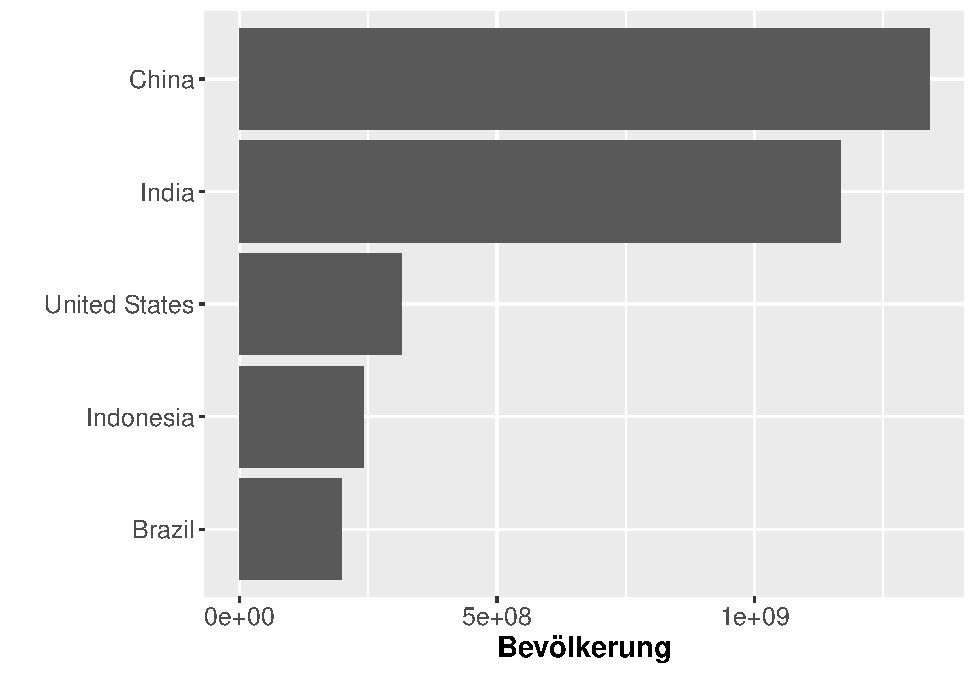
\includegraphics[width=1\linewidth]{PDF_Latex_files/figure-latex/unnamed-chunk-4-1}

Lorem ipsum dolor sit amet, consetetur sadipscing elitr, sed diam nonumy eirmod tempor invidunt ut labore et dolore magna aliquyam erat, sed diam voluptua. At vero eos et accusam et justo duo dolores et ea rebum. Stet clita kasd gubergren, no sea takimata sanctus est Lorem ipsum dolor sit amet. Lorem ipsum dolor sit amet, consetetur sadipscing elitr, sed diam nonumy eirmod tempor invidunt ut labore et dolore magna aliquyam erat, sed diam voluptua. At vero eos et accusam et justo duo dolores et ea rebum. Stet clita kasd gubergren, no sea takimata sanctus est Lorem ipsum dolor sit amet.
\columnbreak

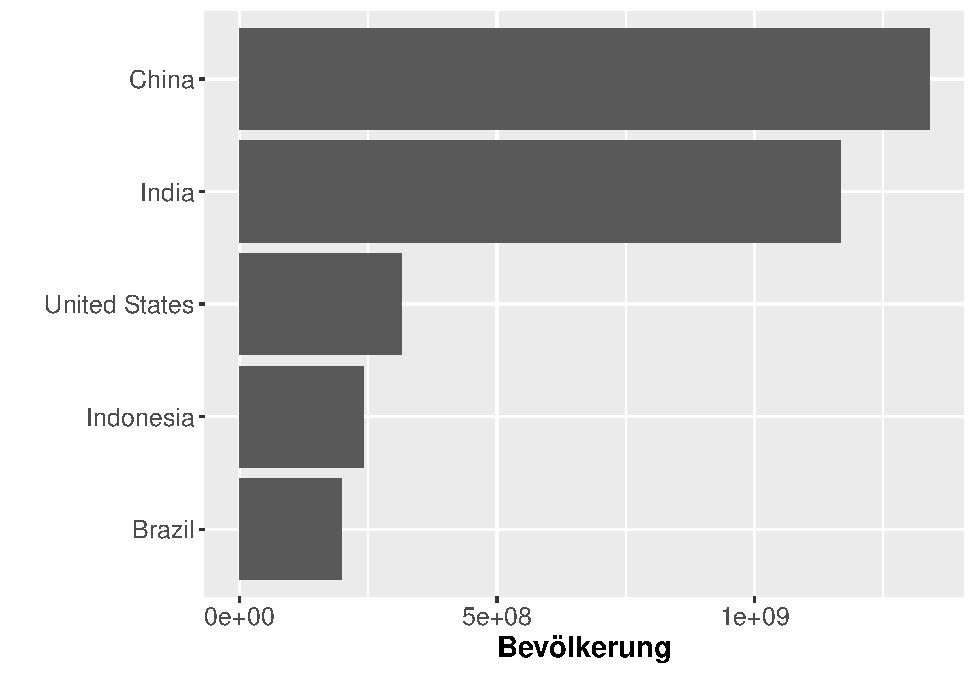
\includegraphics[width=1\linewidth]{PDF_Latex_files/figure-latex/unnamed-chunk-5-1}

Lorem ipsum dolor sit amet, consetetur sadipscing elitr, sed diam nonumy eirmod tempor invidunt ut labore et dolore magna aliquyam erat, sed diam voluptua. At vero eos et accusam et justo duo dolores et ea rebum. Stet clita kasd gubergren, no sea takimata sanctus est Lorem ipsum dolor sit amet. Lorem ipsum dolor sit amet, consetetur sadipscing elitr, sed diam nonumy eirmod tempor invidunt ut labore et dolore magna aliquyam erat, sed diam voluptua. At vero eos et accusam et justo duo dolores et ea rebum. Stet clita kasd gubergren, no sea takimata sanctus est Lorem ipsum dolor sit amet.

\end {multicols}

Lorem ipsum dolor sit amet, consetetur sadipscing elitr, sed diam nonumy eirmod tempor invidunt ut labore et dolore magna aliquyam erat, sed diam voluptua. At vero eos et accusam et justo duo dolores et ea rebum. Stet clita kasd gubergren, no sea takimata sanctus est Lorem ipsum dolor sit amet. Lorem ipsum dolor sit amet, consetetur sadipscing elitr, sed diam nonumy eirmod tempor invidunt ut labore et dolore magna aliquyam erat, sed diam voluptua. At vero eos et accusam et justo duo dolores et ea rebum. Stet clita kasd gubergren, no sea takimata sanctus est Lorem ipsum dolor sit amet.

\begin{verbatim}
## `summarise()` ungrouping output (override with `.groups` argument)
\end{verbatim}

\begin{table}[H]
\centering
\resizebox{\linewidth}{!}{
\begin{tabular}[t]{lrrrrrr}
\toprule
\multicolumn{4}{c}{ } & \multicolumn{3}{c}{Index} \\
\cmidrule(l{3pt}r{3pt}){5-7}
Kontinent & Bevölkerungsdichte & BIP (pro Kopf) & Lebenserwartung & Wohlbefinden & Ungleichheit & Happy Planet\\
\midrule
\cellcolor{gray!6}{Africa} & \cellcolor{gray!6}{60.4} & \cellcolor{gray!6}{3391.9} & \cellcolor{gray!6}{59.8} & \cellcolor{gray!6}{4.4} & \cellcolor{gray!6}{0.4} & \cellcolor{gray!6}{19.9}\\
Asia & 176.0 & 13605.7 & 71.7 & 5.1 & 0.2 & 27.9\\
\cellcolor{gray!6}{Europe} & \cellcolor{gray!6}{114.6} & \cellcolor{gray!6}{25960.5} & \cellcolor{gray!6}{77.9} & \cellcolor{gray!6}{6.1} & \cellcolor{gray!6}{0.1} & \cellcolor{gray!6}{27.2}\\
North America & 136.3 & 14725.4 & 73.9 & 6.1 & 0.2 & 32.2\\
\cellcolor{gray!6}{Oceania} & \cellcolor{gray!6}{19.4} & \cellcolor{gray!6}{13074.2} & \cellcolor{gray!6}{78.3} & \cellcolor{gray!6}{7.0} & \cellcolor{gray!6}{0.1} & \cellcolor{gray!6}{31.0}\\
\addlinespace
South America & 20.6 & 11045.6 & 74.2 & 6.3 & 0.2 & 32.3\\
\bottomrule
\end{tabular}}
\end{table}

\end{document}
